\section{実験方法}
本節では, 提案手法評価の実験方法について述べる.
実験は以下の3つを行った.
\begin{enumerate}
    \item 実験1 入力速度変化に対する内部状態変化の検証
    \item 実験2 ジェスチャー分類問題における入力速度変化に対するモデル精度評価
    \item 実験3 ロボットマニピュレータ軌道予測問題における速度変化に対するモデル精度評価
\end{enumerate}

実験1では提案手法の原理的な検証を行う.
実験2, 実験3では実問題に対して提案手法を適用し, その速度変化に対する有効性を検証する.


\subsection{実験1 入力速度変化に対する内部状態変化の検証}

入力速度変化に対する提案手法の条件 (\eqrefc{eq:approximation:condition1:result} - \eqrefc{eq:approximation:condition3:result}) は, その導出の仮定で入力スパイクのラプラス変換を1とする仮定を用いている.
また, 計算の簡易化のために, 1つのニューロンにおける入力スパイクと内部状態についてのみ議論を行った.
そのため, この条件によって, ネットワーク構造を持つSNNの内部状態が入力の速度変化に対して, 厳密にタイムスケーリングが生じるとは言えない.
そこで実験1では, 入力スパイクのタイムスケーリングに対して, 提案手法を用いることで, その内部状態がタイムスケーリングに近似できることを実験的に検証する.


\subsubsection{実験概要}
まず, 基準速度 ($a=1.0$) の入力スパイク$o_{base}(t)$を生成する.
このとき, 入力スパイク$o_{base}(t)$の生成は, ポアソン分布を用いて行った.
ポアソン分布を用いたスパイクの生成では, 時刻$t$までに$n$回スパイク (=1) が発生する確率$P[n]$は\eqrefc{eq:poisson:distribution}で表される.
\begin{align}
    P[n] = \frac{\left(\lambda t\right)^n}{n!} e^{-\lambda t} \label{eq:poisson:distribution}
\end{align}
ここで, $\lambda$は入力スパイクの平均発生頻度である.
さらに, 微小時間$\it{\Delta} t$のうちに1回スパイクが発生する確率は, 1次までのマクローリン展開より\eqrefc{eq:poisson:distribution:approximation}で表される.
\begin{align}
    P[1] = \frac{\left(\lambda \it{\Delta} t\right)^1}{1!} e^{-\lambda \it{\Delta} t} = \lambda \it{\Delta} t + o(\it{\Delta} t) \simeq \lambda \it{\Delta} t \label{eq:poisson:distribution:approximation}
\end{align}
本実験では$\it{\Delta} t = 1, \lambda=0.1$を用いて, 基準速度の入力スパイク$o_{base}(t)$の生成を行った.

また, 基準速度に対して$a$倍のタイムスケーリングを行った入力スパイク$o_a(t)$を生成する.
$o_a(t)$の生成は, 基準入力スパイク$o_{base}(t)$における時刻$t$のスパイクを, 時刻$at$におけるスパイクに時間方向に平行移動させることで生成した.
入力速度倍率$a$は, 0.1, 0.2, 0.3, 0.4, 0.5, 0.6, 0.7, 0.8, 0.9, 1.0, 2.0, 3.0, 4.0, 5.0, 6.0, 7.0, 8.0, 9.0, 10.0の20種類の値を用いた.

次に, 生成した入力スパイク$o_{base}(t)$と$o_a(t)$を通常のSNNと提案手法のSNNに入力する.
その後, 基準速度入力に対するSNNの最終層の内部状態$v_{base}(t)$と, $a$倍の速度倍率の入力に対するSNNの最終層の内部状態$v_a(t)$の平均二乗誤差 (Mean Squared Error, MSE)を比較する.
$v_{base}(t)$と$v_a(t)$の誤差が小さくなるほど, 提案手法のSNNの内部状態がタイムスケールに近似できていることを示す.
ここで, 入力速度を変えているため, $v_{base}(t)$と$v_a(t)$の総タイムステップ数は一致しない.
そこで, $v_{base}(t)$を線形補間することで, 内部状態のタイムステップ数に合わせてその誤差の計算を行った.

\subsubsection{評価対象モデル}
以下の5種類のモデルをSNNで構築し, 上記の評価を行った.
これらは, ニューラルネットワークにおいて一般的に用いられることが多いモデル構造である.
\begin{itemize}
    \item Linear
    \item CNN
    \item CNN + Dropout
    \item CNN + BatchNormalization
    \item ResNet
\end{itemize}
Lienarは入力データに対して線形変換を行う最も基本的なニューラルネットワークモデルである。
各入力特徴に対して重みを掛け合わせ、バイアスを加算することで出力を生成する.
CNN (Convolutional Neural Network) は, 畳み込み層とプーリング層を用いて入力データの特徴を抽出するニューラルネットワークモデルである.
画像のような空間方向に複数次元の特徴を持つデータに対して用いられることが多い.
Dropoutは過学習を防ぐための正則化手法の一つである.
学習中にランダムに一部のニューロンの結合重みを0 (=ドロップアウト)にすることで, ネットワークが特定のニューロンに依存することを防ぐ.
BatchNormalizationは各ミニバッチを標準化する手法である.
各層の出力がスケーリングされることで勾配消失問題が緩和され, 学習の安定性と速度が向上する.
ResNetは, 深いニューラルネットワークの学習における勾配消失問題を解決するためのモデル構造である.
入力をそのまま出力に反映させる残差ブロックを持つため, 深いネットワークでも学習が容易になる.
ここで, 通常のResNetの構造はSNNでは用いることが困難なため, MS-ResNet (Membrane Shortcut-ResNet)\cite{msresnet} を用いた.
MS-ResNetはニューラルネットワークの各層の出力ではなく, SNNにおけるシナプス電流をスキップ接続することで, 深いSNNでの学習を可能にしている.

Linear構造は一様分布 (\eqrefc{eq:uniform:distribution}) によって重みを初期化した.
\begin{equation}
    w_{i,j} \sim \mathcal{U}\left(-\sqrt{N}, \sqrt{N}\right) \label{eq:uniform:distribution}
\end{equation}
ここで, $N$は入力ニューロン数である.
また, CNN構造はHeの初期化 (\eqrefc{eq:he:initialization}) に基づく分布によって重みを初期化した.
\begin{equation}
    w_{i,j} \sim \mathcal{N}\left(0, \sqrt{\frac{2}{N}}\right) \label{eq:he:initialization}
\end{equation}
それぞれの構造において, 上記の分布で初期化した10個のモデルを用意し, 1000通りの入力スパイクに対して内部状態のMSEを計算した.

各モデルのネットワーク構造およびパラメータを\tabref{tab:model:parameter:linear} - \tabref{tab:model:parameter:resnet}に示す.
ここで, CNNにおいて$kernel\_size=3, stride=1, padding=1$とした.
また, Dropout層における$dr$はドロップアウト率を表す.
SNNのLIFモデルにおけるパラメータは\tabref{tab:model:parameter:lif}に示したものを全てのモデル構造において用いた.
\begin{table}[htbp]
    \centering
    \caption{Linear構造}
    \label{tab:model:parameter:linear}
    \begin{tabular}{ccc}
        \hline
        \textbf{Input size}& \textbf{Hidden size} & \textbf{Output size}\\
        \hline
        1   & 8, 8 & 1 \\
        \hline
    \end{tabular}
\end{table}

\begin{table}[htbp]
    \centering
    \caption{CNN構造}
    \label{tab:model:parameter:cnn}
    \begin{tabular}{cccc}
        \hline
        \textbf{Layer}& \textbf{Type}&\textbf{Input size} & \textbf{Output size}\\
        \hline
        1   & Conv2d & 2x8x8 & 8x8x8 \\
        2 & AveragePooling2d & 8x8x8 & 8x4x4 \\
        3 & Conv2d & 8x4x4 & 16x4x4 \\
        4 & AveragePooling2d & 16x4x4 & 16x2x2 \\
        5 & Linear & 64 & 32 \\
        6 & Linear & 32 & 16 \\
        \hline
    \end{tabular}
\end{table}

\begin{table}[htbp]
    \centering
    \caption{CNN + Dropout構造}
    \label{tab:model:parameter:cnn:dropout}
    \begin{tabular}{cccc}
        \hline
        \textbf{Layer}& \textbf{Type}&\textbf{Input size} & \textbf{Output size}\\
        \hline
        1   & Conv2d & 2x8x8 & 8x8x8 \\
        2 & AveragePooling2d & 8x8x8 & 8x4x4 \\
        3 & Dropout ($dr=0.3$) & 8x4x4 & 8x4x4 \\
        4 & Conv2d & 8x4x4 & 16x4x4 \\
        5 & AveragePooling2d & 16x4x4 & 16x2x2 \\
        6 & Dropout ($dr=0.3$) & 16x2x2 & 16x2x2 \\
        7 & Linear & 64 & 32 \\
        8 & Linear & 32 & 16 \\
        \hline
    \end{tabular}
\end{table}

\begin{table}[htbp]
    \centering
    \caption{CNN + BatchNormalization構造}
    \label{tab:model:parameter:cnn:batchnormalization}
    \begin{tabular}{cccc}
        \hline
        \textbf{Layer}& \textbf{Type}&\textbf{Input size} & \textbf{Output size}\\
        \hline
        1   & Conv2d & 2x8x8 & 8x8x8 \\
        2 & BatchNormalization & 8x8x8 & 8x8x8 \\
        3 & AveragePooling2d & 8x8x8 & 8x4x4 \\
        4 & Conv2d & 8x4x4 & 16x4x4 \\
        5 & BatchNormalization & 16x4x4 & 16x4x4 \\
        6 & AveragePooling2d & 16x4x4 & 16x2x2 \\
        7 & Linear & 64 & 32 \\
        8 & Linear & 32 & 16 \\
        \hline
    \end{tabular}
\end{table}


\begin{table}[htbp]
    \centering
    \caption{ResNet構造}
    \label{tab:model:parameter:resnet}
    \begin{tabular}{ccccc}
        \hline
        \textbf{Layer}& \textbf{Type}&\textbf{Input size} & \textbf{Output size} & \textbf{Residual block nums}\\
        \hline
        1   & MS-ResNet & 2x8x8 & 8x8x8 & 2\\
        2 & AveragePooling2d & 8x8x8 & 8x4x4 & - \\
        3 & MS-ResNet & 8x4x4 & 16x4x4 & 2\\
        4 & AveragePooling2d & 16x4x4 & 16x2x2 & - \\
        5 & Linear & 64 & 32 & - \\
        6 & Linear & 32 & 16 & - \\
        \hline
    \end{tabular}
\end{table}


\begin{table}[htbp]
    \centering
    \caption{LIFモデルのパラメータ}
    \label{tab:model:parameter:lif}
    \begin{tabular}{ccccc}
        \hline
        $\bm{dt}$& $\bm{v_{rest}}$ & $\bm{v_{th}}$ & $\bm{\tau}$ & $\bm{r}$\\
        \hline
        0.001   & 0.0 & 0.01 & 0.05 & 1 \\
        \hline
    \end{tabular}
\end{table}
\subsection{実験2 ジェスチャー分類問題における入力速度変化に対するモデル精度評価}
提案手法をジェスチャー動画分類問題に適用し, 未学習の入力速度に対するモデル精度評価を行う.

\subsubsection{データセット}
ジェスチャー動画のデータセットとして, SNNの評価で広く用いられる\cite{massa2020efficient}DVSGesture\cite{dvsgesture}を使用した.
DVSGestureはイベントベースビジョンセンサ (DVS128 : \figref{fig:dvs128}) で記録されている.
このセンサでは各ピクセルの輝度変化を非同期に捉え, その変化をイベント$\epsilon$として記録する (\eqrefc{eq:dvs:event}).
\begin{equation}
    \epsilon = (x, y, t, p) \label{eq:dvs:event}
\end{equation}
ここで, $(x, y)$はピクセルの座標, $t$はイベントが発生した時刻である.
また, $p$はイベント強度を表し, ピクセルの輝度変化が正であれば1, 負であれば-1の値を持つ.

イベントベースビジョンセンサによるジェスチャー記録の様子を\figref{fig:dvs:recordview}に示す.
上段が通常のフレームベースカメラで記録したもの, 下段がイベントベースビジョンセンサで記録したものである.
また, 黒色は値が0であることを表し, 青色, 桃色はそれぞれ$p=1, p=-1$のイベントを表す.
イベントは時間的なピクセルの輝度変化を検出するため, ジェスチャーでは動きの多い腕周りのピクセル情報が多く記録される.
% 画像引用元
% https://docs.inivation.com/_static/hardware_guides/dvs128.pdf
\begin{figure}[htbp]
    \centering
    \includesvg[width=0.5\textwidth, inkscapelatex=false]{Static/chap2_sec3_dvs128}
    \caption{DVS128\cite{dvs128fig}}
    \label{fig:dvs128}
\end{figure}

\begin{figure}[htbp]
    \centering
    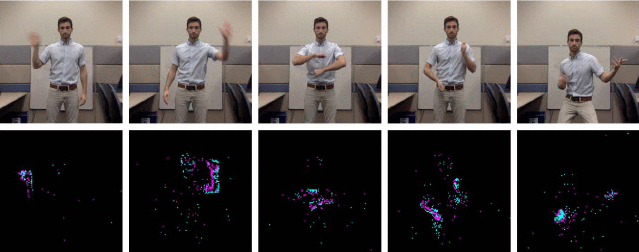
\includegraphics[width=1.0\textwidth]{Static/chap2_sec3_dvs_recordview.png}
    \caption{DVSGesture記録の様子\cite{dvsgesture}}
    \label{fig:dvs:recordview}
\end{figure}

DVSGestureは11種類のクラスのジェスチャーを記録している.
それぞれのジェスチャーのスナップショットを\figref{fig:dvs:gesture}に示す.
\begin{figure}[htbp]
    \centering
    \includesvg[width=0.5\textwidth, inkscapelatex=false]{dummy/dummy_img}
    \caption{各ジェスチャーのスナップショット}
    \label{fig:dvs:gesture}
\end{figure}


\subsubsection{モデルの学習}
モデルの学習はイベントの時系列データを入力, ジェスチャーのクラスを出力とする分類問題として行う.
ここで, 使用するデータセットのイベントの有無をスパイクとして扱うことでSNNの入力としている.

\subsection{実験3 ロボットマニピュレータ軌道予測問題における速度変化に対するモデル精度評価}
提案手法をロボットマニピュレータのエンドエフェクタ軌道予測問題に適用し, 軌道速度変化に対するモデル精度評価を行う.

\subsubsection{実験環境}
実験環境は物理シミュレータであるMujoco\cite{mujoco}を用いた.
また, ロボットマニピュレータは6つの自由度を持つUR5eを用いた.
UR5eの構成図とDenavit-Hartenbergパラメータ (DHパラメータ)をそれぞれ\figref{fig:ur5e:structure}と\tabref{tab:ur5e:dh}に示す.
UR5eの制御は目標手先位置から目標関節角度を逆運動学で求め, PD制御によって行った.
ここで, PD制御におけるPゲイン$K_p$, Dゲイン$K_d$はそれぞれ$1$, $0.1$とした.
また, 目標関節角度の計算はMujocoにおける微分運動学ライブラリであるmink\cite{mink}を用いた.
\begin{figure}[htbp]
    \centering
    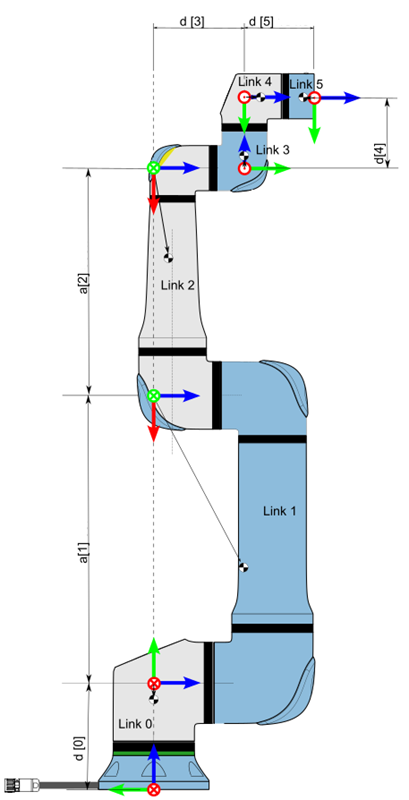
\includegraphics[width=0.5\textwidth]{Static/ur5e_structure.png}
    \caption{UR5eの構成図 \cite{ur5e}}
    \label{fig:ur5e:structure}
\end{figure}

\begin{table}[htbp]
    \centering
    \caption{UR5eのDHパラメータ \cite{ur5e}}
    \label{tab:ur5e:dh}
    \begin{tabular}{ccccc}
        \hline
        \textbf{Joint} & $\bm{\theta}$ [rad] & $\bm{a}$ [m]& $\bm{d}$ [m]& $\bm{\theta}$ [rad]\\
        \hline
        1 & 0 & 0       & 0.1625 & $\pi/2$\\
        2 & 0 & -0.425  & 0       & 0\\
        3 & 0 & -0.3922 & 0       & 0\\
        4 & 0 & 0       & 0.1333 & $\pi/2$\\
        5 & 0 & 0       & 0.0997 & $-\pi/2$\\
        6 & 0 & 0       & 0.0996 & 0\\
        \hline
    \end{tabular}
\end{table}


\subsubsection{モデルの学習}
マニピュレータの関節角度の時系列データ$\bm{q}_{t-T \sim t}$を入力, 次の時刻の目標のエンドエフェクタの位置変化量$\bm{dx}_{t}$を出力とするニューラルネットワークを学習する (\eqrefc{eq:model:learning}).
\begin{equation}
    \bm{dx}_{t} = f_{\theta}(\bm{q}_{t-T \sim t}) \label{eq:model:learning}
\end{equation}
ここで, $f_{\theta}$はニューラルネットワーク, $T$は時系列の長さを表す.
目標軌道は$xy$平面における8の字軌道とし, その軌道は\eqrefc{eq:model:target_trajectoryx}, \eqrefc{eq:model:target_trajectoryy}で表される.
\begin{equation}
    x_t=0.25 \sin (\frac{\pi}{5} t) \label{eq:model:target_trajectoryx}
\end{equation}
\begin{equation}
    y_t=0.075 \sin (\frac{2\pi}{5} t) \label{eq:model:target_trajectoryy}
\end{equation}
本実験では1ステップあたりの時間間隔を$0.07$ s, シーケンス全体が$250$ sの軌道を学習に用いた.
また, $z$座標は$z=0.3$ mで固定した.

% 入力
入力であるマニピュレータの関節角度$\bm{q}$は連続値であるため, SNNに入力するために0か1のスパイクに変換する必要がある.
本実験ではスパイク変換のエンコーダとしてThreshold Encodingを用いた.
このエンコーダは, 入力の変化がある閾値$q_{th}$を超えたときに1を出力し, それ以外の場合は0を出力するものである.
ここで, 閾値$q_{th}$を$q_{th}^{max}$から$q_{th}^{min}$までの範囲で$N_{th}$個に分割することで, 入力の変化を$N_{th}$チャンネルのスパイクとして表現することができる.
本実験では入力関節角度は正規化し, $q_{th}^{max}=1.1$, $q_{th}^{min}=-1.1$, $N_{th}=200$とした.

% モデルタイプ
学習させるモデルは通常のSNNおよび提案手法のSNNとした.
それぞれのモデル構成は大きく2つに分けられ, 1つはSNNによる特徴抽出器$f_{\theta}^{SNN}$, もう一つはNNによる予測器$f_{\theta}^{NN}$である.
SNNの出力は0か1のスパイクであるため, 連続値であるエンドエフェクタ座標を直接予測することは困難である.
そこで, 本実験ではSNNを時系列入力の特徴抽出器として扱う.
さらに, SNNの最終層の内部状態$\bm{v}$を特徴量として, 通常のNNで構成された予測器に入力する.
そして, NNによる予測器が教師エンドエフェクタの座標との誤差が小さくなるようにモデルの学習を行う.
ここで, SNNの最終層の内部状態閾値$v_{th}$は無限大とし, 内部状態がリセットされないようにした.
これはSNNのみでVariational Autoencoder (VAE)を構築したFully Spiking VAE (FSVAE)\cite{fsvae}を参考にした構造である.
また, NN予測器の活性化関数はReLU関数とした.
モデルサイズと学習時のパラメータを\tabref{tab:exp3:model:snn} - \tabref{tab:exp3:train:parameter}に示す.
\begin{table}[htbp] %\20241112\\eight_figure_shallow3\\snn_beta0.95_seq50",
    \centering
    \caption{マニピュレータ軌道予測モデル : SNN特徴抽出器$f_{\theta}^{SNN}$}
    \label{tab:exp3:model:snn}
    \begin{tabular}{ccc}
        \hline
        \textbf{Input size}& \textbf{Hidden size} & \textbf{Output size}\\
        \hline
        1200   & 512, 256, 128 & 128 \\
        \hline
    \end{tabular}
\end{table}

\begin{table}[htbp]
    \centering
    \caption{LIFモデルのパラメータ}
    \label{tab:exp3:model:parameter:lif}
    \begin{tabular}{ccccc}
        \hline
        $\bm{dt}$& $\bm{v_{rest}}$ & $\bm{v_{th}}$ & $\bm{\tau}$ & $\bm{r}$\\
        \hline
        0.03   & 0.0 & 0.1 (最終層のみ$\infty$) & 0.6 & 1 \\
        \hline
    \end{tabular}
\end{table}

\begin{table}[htbp] %\20241112\\eight_figure_shallow3\\snn_beta0.95_seq50",
    \centering
    \caption{マニピュレータ軌道予測モデル : NN予測器$f_{\theta}^{NN}$}
    \label{tab:exp3:model:nn}
    \begin{tabular}{ccc}
        \hline
        \textbf{Input size}& \textbf{Hidden size} & \textbf{Output size}\\
        \hline
        128   & 64, 64, 64 & 2 \\
        \hline
    \end{tabular}
\end{table}

\begin{table}[htbp]
    \centering
    \caption{モデルの学習条件}
    \label{tab:exp3:train:parameter}
    \begin{tabular}{cc}
        \hline
        学習率 $lr$ & 0.001\\
        バッチサイズ $batch\_size$ & 64\\
        エポック数 $epoches$ & 200\\
        勾配クリッピング $clip\_norm$ & 1.0\\
        optimizer & Adam\\
        \hline
    \end{tabular}
\end{table}

学習時の損失関数を\eqrefc{eq:exp3:loss}に示す.
\begin{align}
    \bm{v}^{t,L} &= f_{\theta}^{SNN}(\bm{q}_{t}) \notag \\
    \bm{\hat{dx}}_{t} &= f_{\theta}^{NN}(\bm{v}^{t,L}) \notag \\
    \mathcal{L_{MSE}} &= \frac{1}{T} \sum_{t=1}^{T} \left( \bm{dx}_{t} - \bm{\hat{dx}}_{t} \right)^2 \label{eq:exp3:loss}
\end{align}
ここで, $\bm{v}^{t,L}$は時刻$t$におけるSNNの最終層の内部状態, $\bm{\hat{dx}}^{t}$は時刻$t$における予測器の出力, $\bm{dx}^{t}$は時刻$t$における目標エンドエフェクタ座標である.
また, 損失関数$L_{MSE}$は入力シーケンスの全ての時刻における予測器の出力と教師データの二乗誤差の平均である.


\subsubsection{評価方法}
学習済みのモデルを用いて, 軌道速度変化に対するモデル精度評価を行う.
軌道速度変化は\eqrefc{eq:exp3:target_trajectoryx}によって行う.
\begin{equation}
    \bm{x}_{t+1}^{target} = \bm{x}_{t} + \frac{\bm{\hat{dx}}_{t}} {a} \label{eq:exp3:target_trajectoryx}
\end{equation}
ここで, $\bm{x}_{t}$は現在のエンドエフェクタの座標, $\bm{\hat{dx}}_{t}$はモデルの出力, $\bm{x}_{t+1}^{target}$は目標のエンドエフェクタ座標である.
また, $a$は軌道速度変化倍率である.
速度倍率$a$は0.1, 0.2, 0.3, 0.4, 0.5, 0.6, 0.7, 0.8, 0.9, 1.0, 2.0, 3.0, 4.0, 5.0とした.
それぞれの速度倍率に対して4周期分の軌道を予測および制御を行い, その軌道と目標軌道のMSEを評価した.


